\chapter{Context and importance of this research}
This chapter covers the basic context of the research, regarding the location and past studies of the Yolngu calendar;
finds a gap in the literature and surveys relevant fields;
and lays out the overarching methodology of and strategy for this research.


\section{Context}
% Why does this research matter?  Why do it now?

My guiding research questions are therefore:
\blockquote{
What Yolngu seasonal calendars are generally recognised?\\
Which best affords cross-cultural collaboration?\\
What are the properties and changes that define this calendar?\\
How may these seasons be characterised with respect to temporal and physical patterns in climate?\\
What, if anything, about these seasons is changing in the historical record?\\
What might happen under future climate change?\\
}

I build on existing literature and primary research by deriving a physical characterisation of the Yolngu calendar,
combining traditional Indigenous knowledge with numerical climate science.
Using threshold values in meteorological variables rather than a predefined date range enables
analysis of means and variation in the timing of onset, duration of seasons, and annual patterns in climatological variables.
Preliminary work suggests that these definitions can also be applied to reconstructed or modelled climate data,
allowing investigation of trend or abrupt changes over time.
Well-founded definitions may allow scenario-based investigation of a wider range of conditions than exist in the historical record.

\begin{figure}[h]
    \centering
    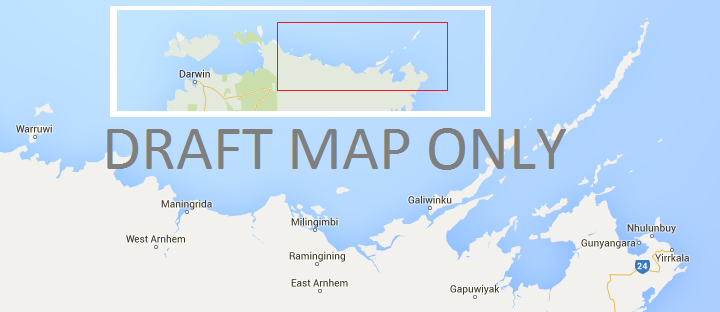
\includegraphics[width=\textwidth]{mapdraft.png}
    \caption[Map showing the study area, NE Arnhem Land]{
        Map showing the study area, NE Arnhem Land.
        Analysis in \autoref{ch:quantify} uses weather observations from several of the towns shown.
        }
    \label{fig:arnhem-map}
\end{figure}

Figure~\ref{fig:arnhem-map} shows the study area in north-east Arnhem Land in Australia.



\section{Literature Review}
\label{sec:lit-review}

After -detailed search strategy-, I was unable to identify any studies which quantified indigenous Australian seasons.
I thus review a number of related fields, explaining the relevance of each and drawing together a summary of this 'gap at the intersection'.
MUST have table here pointing to other parts of the literature review, explaining that concrete parts are in the related methods section to avoid misunderstanding. 
Possible sections – to be reorganised and mutated:

\begin{itemize}
\item Cross cultural and qualitative methods
\item Tropical seasonality, including monsoon and ENSO
\item Anticipated benefits and applications of the research
\item Relationship to phenology and historical climate change
\item Indigenous seasons literature (summary, also compare and contrast)
\item Overview of calendars and seasons – what are they and how are they defined?
\end{itemize}

\section{Methodology and Research Framework}
Explain the structure and relationship of sections 2-4, and how they tie together.
Methods are in each section, but a coherent methodology for the whole thing goes here.
Includes the reason for sections and for each section, ie overall strategy that the research executes.



